\chapter{Implementation of Hindi Question Answer System}

\paragraph{}
This chapter discusses about the different stages involved in the functioning of the  Question Answer System in Yioop. The inputs to the system are the summaries of the web pages Yioop has crawled. For any given page, the summary is processed  by removing punctuation, special characters, etc. After this initial processing, Yioop extracts phrases from the summary which are then subjected to the following modules.

\begin{enumerate} 
\item Part of Speech Tagger.
\item Triplet Extraction i.e Subject, Object, Verb extraction.
\item Named Entity Addition to Database
\end{enumerate}

\section{Part of Speech Tagger}
\paragraph{}
A part of speech tagger plays an important role in natural language translation. Part of speech tagging is also known as word category distribution or grammatical tagging. Tags are basically parts of speech like noun, adjective, verb, etc.   A robust part of speech tagger  can not only retrieve information more efficiently but can also help in understanding what the text actually means. Even with all the advances in machine learning automatic tagging of words  is daunting as many times even hand tagging sentences is difficult purely because of the ambiguous nature of languages. Having said that there are systems designed to perform this task. One such Part of Speech tagger is the Brill tagger  \cite {brill1992simple} which is nothing but a Rule Based Approach to tagging a sentence. Below are the approaches for part of speech tagging, 

\begin{enumerate}
\item Rule Based Approach \\
This is one of the earliest approaches followed to implement tagging. In this approach, we have a set of well-defined rules which are applied to a sentence. The approach uses labelled data which is a lexicon or a dictionary of words and its probable parts of speech. 
The rules are then applied to define the most accurate tag for that word. Ambiguity between multiple tags is sorted by using the tags of words which precede the particular word.
	
\item Machine Learning Based Approach \\
Today we have multiple machine learning algorithms which are used for Part of Speech tagging  \cite {brill1999unsupervised}. Algorithms like Hidden Markov Model, Neural Networks, etc. are trained on a small sample of text and over time these models prove to be almost as effective in retrieving information as a human would do. The most known part of speech tagging algorithms apart from Brill Tagging are the Viterbi Algorithm.
\end{enumerate}

\paragraph{}
We have an implementation of a Brill tagger for English and a similar variant for Hindi \cite {garg2012rule}, \cite {dalal2006hindi}.  The initial implementation of the Question Answer System had a file based lexicon which meant tagging a word required a file scan, which eventually  slowed the Question Answer module in Yioop as a whole. As a solution, the lexicon is now stored as part of the database which will be used by Yioop. The lexicon table created is indexed on the word and locale meaning the retrieval time is reduced to $O(1)$ greatly improving the speed of the Question Answer module. 

\paragraph{}
For the Hindi variant of the Brill tagger, we first tag the words as per data available in the database. Then for the remaining words of the sentence we use the rules to assign the most probable tag. On the next page, we describe the algorithm and the rules used to tag words in a Hindi Sentence.  \\

\break
\begin{enumerate}
\item Use the Lexicon in the database \\
First tag the words in the phrase which are present in the Lexicon. The words which are not present in the lexicon are tagged as Unknown. We then apply the below rules to tag the words.

\item{Rule to identify Noun} \\
RULE 1: If the previous word tagged is an Adjective / Pronoun / Postposition then the current word is likely to be a noun \\	
RULE 2: If the current word is a verb then the previous word is a noun \\
RULE 3: If the current tag is a noun then next / previous is a noun
		
\item{Rule to identify demonstrative nouns} \\
RULE 1: If the current and previous words are tagged as pronouns then the previous word is a demonstrative \\
RULE 2: If the current word is a noun and the previous word is a pronoun then the current word is demonstrative
		
\item{Rule to identify pronoun} \\
RULE: If the previous word is unknown and the current word is a noun then the previous word is a pronoun
		
\item{Rule to identify Noun} \\		
RULE: If we get two words which are untagged the most probably they form a name and will be tagged as noun
		
\item{Rule to identify Adjective} \\
RULE: If the word ends with <tar>, <tam>, <thik> then we tag it as a Adjective
		
\item{Rule to identify verbs} \\
RULE: If the current word is tagged as Auxilary verb  and the previous word is tagged as Unknown then  the previous word is a verb

\item{No rule matched} \\
RULE: After applying all the rules if the word is still tagged as Unknown then tag it as a Noun.
		
\end{enumerate}
	
\begin{algorithm}
\caption{Part of Speech Tagger}\label{alg:brilltaggervariant}
\begin{algorithmic}[1]
\Procedure{tagpartofSpeech}{$sentence$}
\State terms $\gets$ sentence split on space 
\State result $\gets$ []
\State i $\gets$ 0
\For { term in terms }
\State term['tag'] $\gets$ unknown
\State partofspeech $\gets$ select partofspeech from database where word $\gets$ term
\If {partofspeech exists} 
\State term['tag'] $\gets$ partofSpeech 
\EndIf
\State result[i++] = term
\EndFor
\State result = tagUnknowWords(result)
\State return result
\EndProcedure

\Procedure{tagUnknownWords}{$partially tagged sentence$}
\For {term tagged as Unknown} 
\If {$previous['tag'] \gets Adjective$ OR $previous['tag'] \gets Pronoun$ OR $previous['tag'] \gets Participle$ }
\State current['tag] $\gets$ noun
\State result $\gets$ current
\EndIf
\If {$current['tag'] \gets verb$ }
\State previous['tag] $\gets$ noun
\State result $\gets$ previous
\EndIf		
\algstore{myalg}		
\end{algorithmic}
\end{algorithm}
\begin{algorithm}
\caption{Part of Speech Tagger}\label{alg:brilltaggervariant}              
\begin{algorithmic}                 
\algrestore{myalg}
\If {$previous['tag'] \gets unknown$  AND $current['tag'] \gets noun$ }
\State previous['tag] $\gets$ pronoun
\State result $\gets$ previous
\EndIf
\If {$current['tag'] \gets aux. verb$ OR $previous['tag'] \gets unknown$ }
\State previous['tag] $\gets$ verb
\State result $\gets$ previous
\EndIf
\If {current['token'] ends with 'eek' OR current['token'] ends with 'tar' OR current['token'] ends with 'tam'}
\State current['tag'] $\gets$ adjective
\State result $\gets$ current
\EndIf
\If {$current['tag'] \gets unknown$}
\State  current['tag] $\gets$ noun
\State result $\gets$ current
\EndIf
\EndFor
\State return result
\EndProcedure
\end{algorithmic}
\end{algorithm}
\break

\section {Parse Tree Generation}
\paragraph{}
After all the words in the sentence are tagged with the most probable part of speech, we generate a tree like structure composing of the Noun, Verb and PostPosition or Preposition Phrase. For a Hindi sentence \cite{bhat2017improving}, the structure is generally Noun Phrase followed by the Verb Phrase, which is same as most of the English sentences. In English, the verb or the predicate helps us separate the Noun and Verb Phrase, in case of Hindi we have something similar, these are known as $case$ words. These help us distinguish between the subject and object in a given sentence. This is the reason we have implemented the Hindi parse tree to be comprised of Noun Phrase, Postposition Phrase and Verb Phrase. 

\textbf {NP: $\{ \langle$ JJ | NN* $\rangle \}$+}  \\

For any given sentence, the initial sequence of adjectives and nouns becomes part of the noun phrase. The next step is to extract the post positional or the prepositional phrase following the noun phrase this will form the object of the sentence,

\textbf {PP: $\{ \langle$ IN | JJ | NN | PP $\rangle \}$+} \\

This rule extracts the information from the sentence till we encounter the verb phrase. Hindi being a subject-object-verb language, most of the sentences usually end with verbs. So the verb phrase extraction rule is \\

\textbf {VP: $\{ \langle$ VB*$\rangle \langle $ IN | NP $\rangle \}$} \\

In Hindi, the case words which separate the noun and post position phrase are the ones which help define the relationship between the subject and object. Hence, identifying the case words more accurately will help increase how accurate the generated parse tree will be. Below we describe the algorithms for parsing the sentence for different parts like the Noun Phrase, Postpositional Phrase and Verb Phrase,

\begin{figure}[htb]
\centering
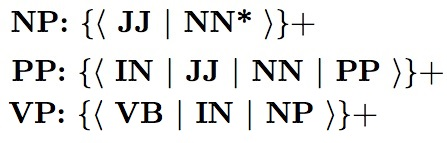
\includegraphics[width=0.5\textwidth]{images/gammarrules.jpg}
\caption{Grammar Rules.} 
\label{fig:gammarrules}
\end{figure}

\begin {algorithm}
\caption {Extract Noun Phrase}
\begin {algorithmic}[1]
\Procedure{extractNounPhrase}{$taggedPhrase, parseTree$}
\State curNode $\gets$ parseTree[node]
\State adjectiveTree $\gets$ extractAdjective from the tagged phrase from currentNode
\State currentNode $\gets$ just after the node last processed by extractAdjective
\State nounTree $\gets$ extractNouns from the tagged phrase from currentNode
\State tree $\gets$ adjectiveTree $\cup$ nounTree 
\State return tree
\EndProcedure		
\end {algorithmic}
\end {algorithm}

\begin {algorithm}
\caption {Extract Post Positional Phrase}
\begin {algorithmic}[1]
\Procedure{extractPostpositionPhrase}{$taggedPhrase, parseTree$}
\State currentNode $\gets$ parseTree[node]
 \If {$current['tag']$ is post position}
 \State postPositionTree $\gets$ extractpostposition from the tagged phrase from currentNode
\State currentNode $\gets$ just after the node last processed by extractpostposition
\State adjectiveTree $\gets$ extractAdjective from the tagged phrase from currentNode
\State currentNode $\gets$ just after the node last processed by extractAdjective
\State nounTree $\gets$ extractNouns from the tagged phrase from currentNode
\State extractPostpositionPhrase with updated currentNode extract information until verb is encountered
\EndIf
\State return tree
\EndProcedure		
\end {algorithmic}
\end {algorithm}

\begin {algorithm}
\caption {Extract Verb Phrase}
\begin {algorithmic}[1]
\Procedure{extractVerbPhrase}{$taggedPhrase, parseTree$}
\State currentNode $\gets$ parseTree[node]
\State verbTree $\gets$ extractVerbs from the tagged phrase from currentNode
\State postPositionTree $\gets$ extractpostposition from the tagged phrase from currentNode
\State nounphrasetree $\gets$ call extractNounPhrase
\State return tree
\EndProcedure		
\end {algorithmic}
\end {algorithm}

\section{Triplet Extraction}
\paragraph{}
Phrases in languages like English and Hindi are mainly composed of three parts viz. the Subject, Object and Verb. The triplet extraction module is responsible for retrieving these parts from a phrase, which are then rearranged to form multiple question answer pairs.

\paragraph{}
After a given sentence has all the words tagged with its most probable part of speech we generate a tree like structure known as the parse tree which is made of the Noun Phrase and Verb Phrase. In case of Hindi, we have  three parts to the parse tree the Noun Phrase, PostPosition Phrase and the Verb Phrase. We do this because English being a Subject-Verb-Object language, the triplet extractor is able to extract the subject, verb, object triplet from the Noun and Verb Phrase. Incase of Hindi, which is a Subject-Object-Verb language, we use the PostPosition Phrase to help us distinguish between the Subject and the Object in a given sentence. We describe the triplet extraction algorithm which takes as input the parse tree and returns a triplet.

\begin {algorithm}
\caption {Triplet Extraction}
\begin {algorithmic}[1]
\Procedure{tripletextraction}{$parseTree$}
\State triplet $\gets$ extractSubject(parseTree) $\cup$ extractObject(parseTree) $\cup$ extractVerb(parseTree)
\State return triplet
\EndProcedure		
\end {algorithmic}
\end {algorithm}

\paragraph{Subject Extraction}
We extract the subject from the parse tree by recursively parsing the noun phrase for the first level noun, this constitutes the subject for a CONCISE triplet, we then continue to parse the entire noun phrase from the parse tree to form the subject for the RAW version of the triplet. The RAW version of the triplet consists of words tagged as JJ, NN, NNP, NNP, NNPS. The CONCISE form of the triplet consists only of the first level noun this results in lose of some information from the text. On the other hand, the RAW triplet consists of the adjectives in the noun phrase which helps preserve the information.

\paragraph{Object Extraction}
The next step is extracting the object from the parse tree. We achieve this by parsing the postposition phrase in the parse tree. The object constitutes to the remaining nouns in the sentence. For a hindi sentence, the object is responsible for providing the answers to most of the wh questions like who, where, when etc. For example, a question in English like "Who is Barack Obama"  becomes "Barack Obama kaun hai", here the word 'kaun' represents the 'Who' in the question, the answer to which is stored by the object. Another example, "When is the new year" becomes "Naya saal kab hai"  here "kab" represents the "when" in the question and is answered to by the corresponding object stored as part of the triplet.

\paragraph{Predicate Extraction}
The predicate is extracted from the Verb phrase of the parse tree. These are terms tagged with VB, VBZ, VBG, VBP. As compared to a English sentence, the verb phrase has minimal information related to the text. It helps define the tense and relation between the information extracted from subject and object.

\section{Named Entity Addition}
The performance of the Question Answer system depends on the ability to extract information from the text. As we know most of the answers are facts (named entities) for such a system, the accuracy of the system is directly proportional to its ability to recognize them from the text. Most of the existing systems use a hand written dictionary of named entities to enhance the results. Following a similar approach, we add an option under the Page Options section in Yioop for the user to add entities to the Lexicon table. The user can do this by adding a single entity at a time as shown below in Figure~\ref{fig:named_entity_manual} 

\begin{figure}[htb]
\centering
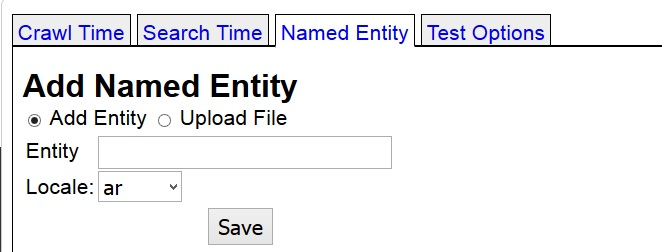
\includegraphics[width=0.8\textwidth]{images/named_entity_manual.jpg}
\caption{Add Named Entity.} 
\label{fig:named_entity_manual}
\end{figure}

Or they can upload a text file to Yioop which contains line separated entities and select the locale for the which the file contains the entities as shown in Figure~\ref{fig:named_entity_file} 

\begin{figure}[htb]
\centering
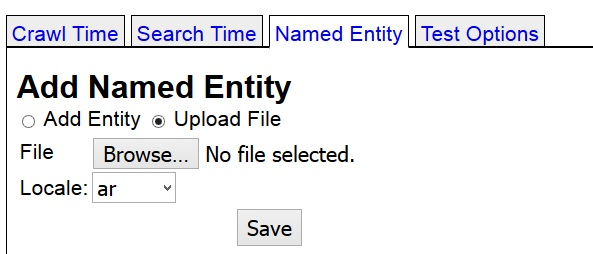
\includegraphics[width=0.8\textwidth]{images/named_entity_file.jpg}
\caption{File Upload to add Named Entities.} 
\label{fig:named_entity_file}
\end{figure}

For any given language user can view all the entities already added to the database, they can edit or delete entities of their choice. The UI for this functionality is as shown in Figure~\ref{fig:viewallentities}

\begin{figure}[htb]
\centering
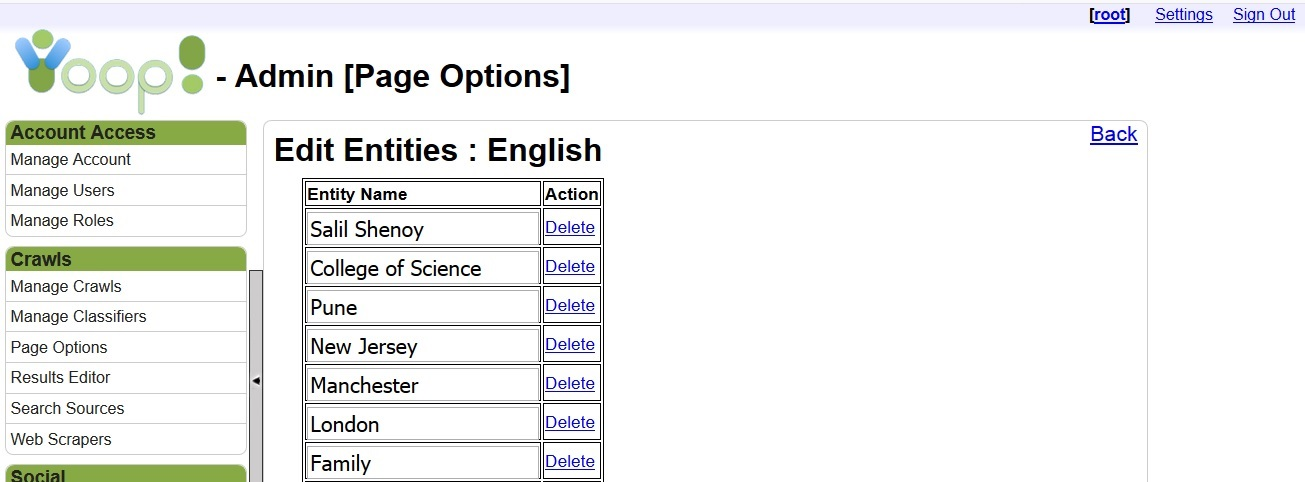
\includegraphics[width=0.8\textwidth]{images/viewallentities.jpg}
\caption{View all Entities.} 
\label{fig:viewallentities}
\end{figure}
